% 柯西积分定理
% 柯西—古萨定理|环路积分|积分路径|解析函数

\pentry{复变函数的积分\upref{CpxInt}}

% 我们知道复变函数的积分可以看成二维平面上某个矢量场的线积分

在复变函数的积分\upref{CauGou}里的例子可以发现,有的函数的积分只依赖于积分路径的起点与终点,而与积分路径的形状无关,而有的函数,其积分不仅与积分路径的起点与终点有关,而且与积分路径的形状也有关.深入观察后,可知,前一类函数是解析函数.由此,可提出猜想:解析函数的积分只依赖于积分路径的起点与终点,而与积分路径的形状无关.柯西在1825年给出此定理对猜想作了回答.也就是我们现在要介绍的\textbf{柯西积分定理(Cauchy's integral theorem)}, 也叫\textbf{柯西—古萨定理(Cauchy–Goursat theorem)}.

\begin{theorem}{柯西积分定理}
设$G $为复平面上的单连通区域,$C $为$G $内的任意一条围线,如图所示,若$f (z)$在$G $内解析,则
\begin{equation}
\oint_{C} f(z) \mathrm{d} z=0
\end{equation}
\begin{figure}[ht]
\centering
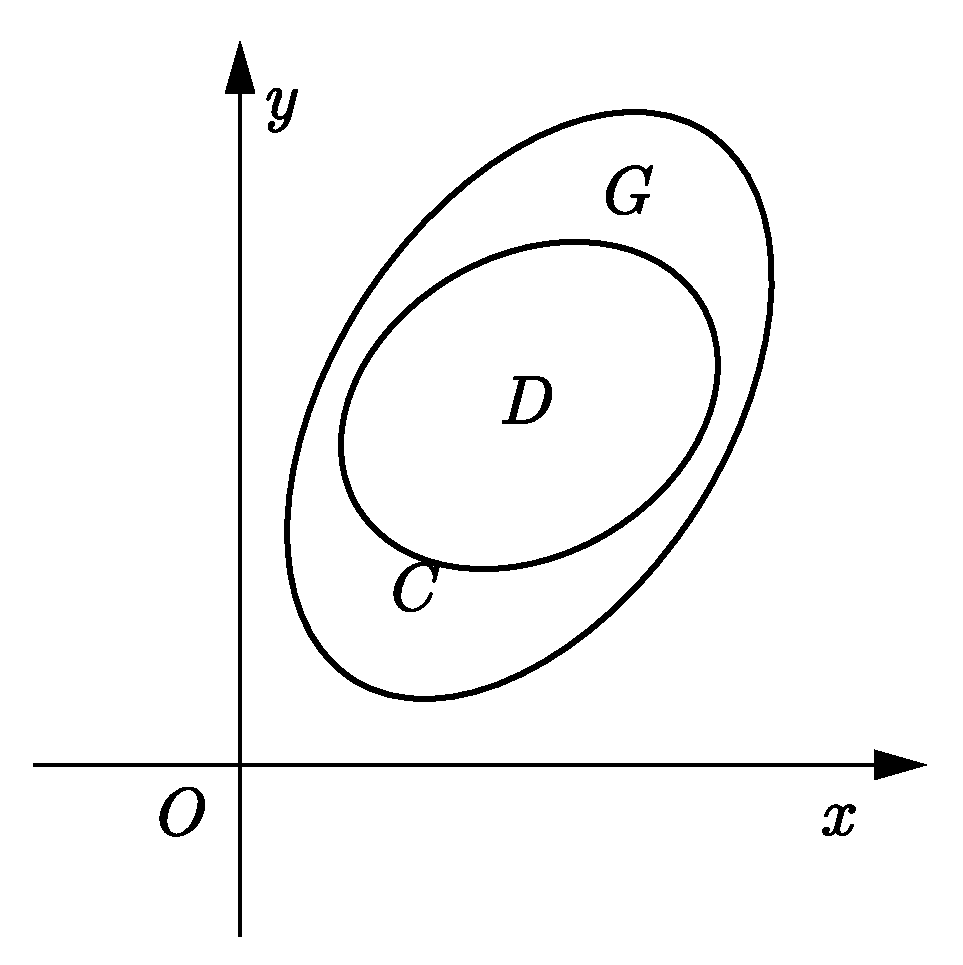
\includegraphics[width=5cm]{./figures/CauGou_1.pdf}
\caption{积分回路} \label{CauGou_fig1}
\end{figure}

下面为了简单起见,在假设$f'(z)$连续的情况下证明该定理,也就是黎曼在1851年给出的证明方法.

令$z=x+\mathrm{i} y, f(z)=u(x, y)+\mathrm{i} v(x, y)$,我们有
\begin{equation}
\oint_{C} f(z) \mathrm{d} z=\oint_{C} u \mathrm{d} x-v \mathrm{d} y+\mathrm{i} \oint_{C} v \mathrm{d} x+u \mathrm{d} y
\end{equation}
由于$f^{\prime}(z)=u_{x}+\mathrm{i} v_{x}=v_{x}-\mathrm{i} u_{y}$在$G $内连续,所以,$u_{x}, u_{y}, v_{x}, v_{y}$在$G $内连续,从而,这四个偏导数在由围线$C$及其内部构成的闭区域$D $上连续.又因$C $为光滑或逐段光滑的闭曲线,且$u $与$v $在$D $上连续是显然的.于是,由高等数学中的格林公式或斯托克斯定理\upref{Curl}得
\begin{equation}\label{CauGou_eq1}
\begin{aligned}\oint_C u \mathrm{d} x-v \mathrm{d} y=\iint_{D}\left(-v_{x}-u_{y}\right) \mathrm{d} x \mathrm{d} y \\ \oint_C v \mathrm{d} x+u \mathrm{d} y=\iint_{D}\left(u_{x}-v_{y}\right) \mathrm{d} x \mathrm{d} y\end{aligned}
\end{equation}
而由$ f (z)$在G 内解析知道,$u$与$v$满足柯西—黎曼条件(\autoref{CauRie_eq1}~\upref{CauRie})
\begin{equation}
u_{x}=v_{y}, \quad u_{y}=-v_{x}
\end{equation}
由此得\autoref{CauGou_eq1} 中两个积分都为零, 即
\begin{equation}
\oint_{C} f(z) \mathrm{d} z=0
\end{equation}
\end{theorem}
这个定理其实也提供了一种计算解析函数沿围线积分的方法.下面来看一道例题.
\begin{example}{}
计算积分
\begin{equation}
\oint_{|z+1|=\frac{1}{4}} \frac{3 z}{(z-2)(z-1)} \mathrm{d} z
\end{equation}
作区域$G:|z+1|<1$,显然,积分路径$|z+1|=1/4$位于$G$内,由柯西积分定理, 积分结果为 0.
\end{example}
